\documentclass[paper=letter, fontsize=11pt]{scrartcl} 

\usepackage{graphicx}
\usepackage{verbatim}
\usepackage{pictex}  
\usepackage{multimedia}
\usepackage{listings}
\usepackage{xcolor,colortbl}
\usepackage[spanish]{babel} % language/hyphenation
\usepackage[utf8]{inputenc}
\usepackage{amsmath,amsfonts,amsthm} % Math packages
\usepackage{dirtytalk}
\usepackage{color}
\usepackage{amsbsy}
\usepackage{amssymb}
\usepackage{fancyvrb}
\usepackage{sectsty} % Allows customizing section commands
\allsectionsfont{\centering \normalfont\scshape} % Make all sections centered, the default font and small caps

\usepackage{fancyhdr} % Custom headers and footers
\pagestyle{fancyplain} % Makes all pages in the document conform to the custom headers and footers
\fancyhead{} % No page header - if you want one, create it in the same way as the footers below
\fancyfoot[L]{} % Empty left footer
\fancyfoot[C]{} % Empty center footer
\fancyfoot[R]{\thepage} % Page numbering for right footer
\renewcommand{\headrulewidth}{0pt} % Remove header underlines
\renewcommand{\footrulewidth}{0pt} % Remove footer underlines
\setlength{\headheight}{13.6pt} % Customize the height of the header

\numberwithin{equation}{section} % Number equations within sections (i.e. 1.1, 1.2, 2.1, 2.2 instead of 1, 2, 3, 4)
\numberwithin{figure}{section} % Number figures within sections (i.e. 1.1, 1.2, 2.1, 2.2 instead of 1, 2, 3, 4)
\numberwithin{table}{section} % Number tables within sections (i.e. 1.1, 1.2, 2.1, 2.2 instead of 1, 2, 3, 4)

\setlength\parindent{0pt} % Removes all indentation from paragraphs - comment this line for an assignment with lots of text
\lstset{language=R,literate={<-}{{$\gets$}}1}
\newcommand{\horrule}[1]{\rule{\linewidth}{#1}} % Create horizontal rule command with 1 argument of height

\title{	
\normalfont \normalsize 
\textsc{Centro de Investigaci\'on en Matem\'aticas (CIMAT). Unidad Monterrey} 
\\ [25pt] 
\horrule{0.5pt} \\[0.4cm] % Thin top horizontal rule
\huge An\'alisis de datos complejos: Tarea 1\\ 
\horrule{2pt} \\[0.5cm] % Thick bottom horizontal rule
}

\author{Jorge Luis Ramos Zavaleta} % Your name

\date{\normalsize\today} % Today's date or a custom date

\begin{document}
\lstdefinestyle{customc}{
  belowcaptionskip=1\baselineskip,
  basicstyle=\footnotesize, 
  frame=lrtb,
  breaklines=true,
  %frame=L,
  %xleftmargin=\parindent,
  language=C,
  showstringspaces=false,
  basicstyle=\footnotesize\ttfamily,
  keywordstyle=\bfseries\color{green!40!black},
  commentstyle=\itshape\color{red!40!black},
  identifierstyle=\color{blue},
  stringstyle=\color{purple},
}

\lstset{breakatwhitespace=true,
  basicstyle=\footnotesize, 
  commentstyle=\color{green},
  keywordstyle=\color{blue},
  stringstyle=\color{purple},
  language=C++,
  columns=fullflexible,
  keepspaces=true,
  breaklines=true,
  tabsize=3, 
  showstringspaces=false,
  extendedchars=true}

\lstset{ %
  language=R,    
  basicstyle=\footnotesize, 
  numbers=left,             
  numberstyle=\tiny\color{gray}, 
  stepnumber=1,              
  numbersep=5pt,             
  backgroundcolor=\color{white},
  showspaces=false,             
  showstringspaces=false,       
  showtabs=false,               
  frame=single,                 
  rulecolor=\color{black},      
  tabsize=2,                  
  captionpos=b,               
  breaklines=true,            
  breakatwhitespace=false,    
  title=\lstname,             
  keywordstyle=\color{blue},  
  commentstyle=\color{dkgreen},
  stringstyle=\color{mauve},   
  escapeinside={\%*}{*)},      
  morekeywords={*,...}         
} 


\maketitle % Print the title


\section{Ejercicio}
Implementa un corrector ortográfico automático para textos en español.
Dada una palabra w, encuentra la palabra s que (suponemos), es la que se quer\'ia
escribir correctamente. Para esto, considera el siguiente modelo básico:
$$s = arg \max\limits_{s} P (s|w) = arg \max\limits_{s} P (w|s)P (s),$$

donde, $P(s)$ es el modelo del lenguaje, y representa la probabilidad de que la
palabra s sea la que se intentó escribir. La probabilidad $P(w|s)$ representa el
modelo de error o canal ruidoso, e indica la probabilidad de que, por alguna
razón, se escribió la palabra w en lugar de la “correcta” s.

\subsection{Soluci\'on}
Para obtener el corrector ortogr\'afico se considero una distribuci\'on apriori, en este caso dada por dos posibles diccionarios con frecuencias de aparaci\'on de palabras, se uso un diccionario de frecuencia de palabras según el Corpus OpenSubtitles y el diccionario CREA de las 10,000 palabras mas frecuentes.\newline

Para la prueba de nuestro corrector ortogr\'afico se hizo uso del SFU review corpus, que contiene rese\~nas de diversos objetos y servicios, para ello se hizo uso de los dos diccionarios de frecuencias antes mencionados y de un corrector ortogr\'afico conocido como Aspell para comprobar nuestros resultados contra los que se obtienen con Aspell. Hay varias formas de usar Aspell, pero en algunos sistemas Linux viene incluido y puede usarse directamente escribiendo en consola $$aspell \ check \ nombredelarchivo.txt$$ con lo que se activa la consola interactiva. Para hacer comparable el resultado de Aspell se eligi\'o reemplazar las palabras escritas incorrectamente con la primera opci\'on que Aspell ofrec\'ia. \newline

Como parte del preprocesamiento de los textos, se realizo un tokenizacion del texto eliminando puntuaci\'on y n\'umeros del texto para permitirnos trabajar solo con las palabras que son la parte que nos interesa usar para la correcci\'on. \newline

Para la parte de la probabilidad condicional se uso la distancia de Levenshtein, y para reducir el costo computacional se eligieron las palabras contra las cuales se deb\'ia comparar usando 2 criterios. \begin{enumerate}
    \item Las palabras elegidas no deben diferir en mas de dos car\'acter de longit\'ud de la palabra a corregir.
    \item Las palabras elegidas deben coincidir en el primer car\'acter con la palabra a corregir.
    \item Se elige la primera palabra que aparece en la lista que contiene las palabras con el mismo valor del argumento m\'aximo.
\end{enumerate}

Para establecer las probabilidades condicionales solo se consideraron palabras cuya distancia de Levenshtein fuera a lo m\'as dos. Por lo que se estableci\'o la siguiente regla de asignaci\'on de probabilidad con respecto a la distancia obtenida \begin{table}[h]
\centering
\begin{tabular}{ccc}
Distancia &  & Probabilidad asignada\\
0        & $\rightarrow$ & 0.9  \\
1        & $\rightarrow$ & 0.09 \\
2        & $\rightarrow$ & 0.01 \\
Mas de 3 & $\rightarrow$ & 0   
\end{tabular}
\end{table}

Un problema al que nos enfrentamos directamente es que no tenemos inicialmente una m\'etrica para saber que tanto se equivocaron los correctores ortogr\'aficos de manera autom\'atica por lo que la prueba se realizo en solo unas pocas rese\~as para poder hacer una inspecci\'on manual de la correci\'on. A manera de ejemplo se muestran los resultados obtenidos para una rese\~na de un coche (no\_2\_9.txt) resaltando las palabras que fueron corregidas de manera incorrecta.\newline
\newpage
\textbf{Texto original}\newline

\say{En esta opinión voy a hablar del Opel Astra, aunque es una crítica en general a la marca Opel.\newline

Hablo desde mi experiencia, y la de tres amigos míos más. Me explico, yo tuve un Opel Corsa, en el que al final casi tuve que cambiar hasta el volante, ya que se me averió de todo. Pero obviando este asunto, ya que se trataba de un coche viejo y tal... dos amigos míos compraron dos Opel Astra nuevecitos. Uno de ellos en el primer mes tuvo problemas de todo tipo, con los antivaho, con el aire acondicionado, con las luces... El otro, en el año siguiente a su compra, ha tenido muchisimas averías, no le funcionaba el cierre automático del maletero, le saltaban las alarmas de averías en el panel sin tenerlas, una temporada le arrancaba mal y era problema del carburador..., y todo eso en el primer año desde su compra. Y un tercero compró un Opel Vectra, al año se le estropeo el aire acondicionado, y encima no se lo querían reparar porque decían que la culpa era suya por no haberle llevado a la revisión... Al final y ante la amenaza de denuncias accedieron, pero le costó lo suyo.\newline

Por mi propia experiencia, como comprendereis, el próximo coche queme compre no será un Opel...\newline

Saludos.} \newline

\textbf{Texto corregido usando el Corpus OpenSubtitles}\newline

\say{En esta opinión voy a hablar del Opel Astra, aunque es una crítica en general a la marca Opel.\newline

Hablo desde mi experiencia, y la de tres amigos \colorbox{yellow}{mío} más. Me explico, yo tuve un Opel Corsa, en el que al final casi tuve que cambiar hasta el  \colorbox{yellow}{volantes}, ya que se me averió de todo. Pero obviando este asunto, ya que se trataba de un coche viejo y tal... dos amigos  \colorbox{yellow}{mío} compraron dos Opel Astra nuevecitos. Uno de ellos en el primer  \colorbox{yellow}{me} tuvo problemas de todo tipo, con los \colorbox{yellow}{activado}, con el aire acondicionado, con las luces... El otro, en el año siguiente a su compra, ha tenido muchísimas averías, no le funcionaba el cierre automático del maletero, le saltaban las alarmas de averías en el \colorbox{yellow}{papel} sin tenerlas, una temporada le arrancaba mal y era problema del carburador..., y todo eso en el primer año desde su compra. Y un tercero compró un Opel Vectra, al año se le estropeo el aire acondicionado, y encima no se lo quería reparar porque decían que la culpa era suya por no haberle llevado a la revisión... Al final y ante la amenaza de denuncias accedieron, pero le costó lo suyo.\newline

Por mi propia experiencia, como comprenderás, el próximo coche que compre no será un Opel...\newline

Saludos. }\newline

\textbf{Texto corregido usando las 10,000 palabras de la RAE}\newline

\say{En esta opinión voy a hablar del Opel Astra, aunque es una crítica en general a la marca Opel.\newline

Hablo desde mi experiencia, y la de tres amigos \colorbox{yellow}{más} más. Me \colorbox{yellow}{explicó}, \colorbox{yellow}{y} tuve un Opel Corsa, en el que al final casi tuve que cambiar hasta el volante, y que se me \colorbox{yellow}{abrió} de todo. Pero \colorbox{yellow}{objeto} este asunto, \colorbox{yellow}{y} que se trataba de un coche viejo y tal... dos amigos más \colorbox{yellow}{comprar} dos Opel Astra \colorbox{yellow}{nacional}. Uno de ellos en el primer \colorbox{yellow}{más} tuvo problemas de todo tipo, con los \colorbox{yellow}{aunque}, con el aire \colorbox{yellow}{administración}, con las luces... El otro, en el año siguiente a su compra, ha tenido \colorbox{yellow}{mientras} \colorbox{yellow}{ahora}, no \colorbox{yellow}{la} \colorbox{yellow}{funciona} el cierre automático del \colorbox{yellow}{mientras}, \colorbox{yellow}{la siempre} las \colorbox{yellow}{alarma} de \colorbox{yellow}{ahora} en el \colorbox{yellow}{papel} sin \colorbox{yellow}{también}, una temporada \colorbox{yellow}{la arranca} mal y era problema del \colorbox{yellow}{cualquier}..., y todo eso en el primer año desde su compra. Y un tercero compró un Opel Vectra, al año se le \colorbox{yellow}{europeo} el aire \colorbox{yellow}{administración}, y encima no se lo querían reparar porque decían que la culpa era \colorbox{yellow}{su} por no haberle llevado a la revisión... Al final y ante la amenaza de denuncias \colorbox{yellow}{acudieron}, pero le costó lo \colorbox{yellow}{su}.\newline

Por mi propia experiencia, como \colorbox{yellow}{condiciones}, el próximo coche que \colorbox{yellow}{compra} no será un Opel...\newline

Saludos. }\newline

\textbf{Texto corregido con Aspell}\newline

\say{En esta \colorbox{yellow}{opinoón} voy a hablar del \colorbox{yellow}{Piel Astera}, aunque es una \colorbox{yellow}{ceíti ca} en general a la marca \colorbox{yellow}{Piel}.\newline

Hablo desde mi experiencia, y la de tres amigos míos más. Me explico, yo tuve un \colorbox{yellow}{Piel} Corsa, en el que al final casi tuve que cambiar hasta el volante, ya que se me \colorbox{yellow}{averiéó} de todo. Pero obviando este asunto, ya que se trataba de un coche viejo y tal... dos amigos míos compraron dos \colorbox{yellow}{Piel Astera nueve citos}. Uno de ellos en el primer mes tuvo problemas de todo tipo, con los \colorbox{yellow}{anteva}, con el aire acondicionado, con las luces... El otro, en el año siguiente a su compra, ha tenido \colorbox{yellow}{muchísimas aveías}, no le funcionaba el cierre \colorbox{yellow}{átomoátoco} del maletero, le saltaban las alarmas de \colorbox{yellow}{aveías} en el panel sin tenerlas, una temporada le arrancaba mal y era problema del carburador..., y todo eso en el primer año desde su compra. Y un tercero \colorbox{yellow}{compraó} un \colorbox{yellow}{Piel Vector}, al año se le estropeo el aire acondicionado, y encima no se lo \colorbox{yellow}{queraíAna} reparar porque \colorbox{yellow}{deíAna} que la culpa era suya por no haberle llevado a la \colorbox{yellow}{revisoón}... Al final y ante la amenaza de denuncias accedieron, pero le \colorbox{yellow}{costaó} lo suyo.\newline

Por mi propia experiencia, como \colorbox{yellow}{comprenderéis}, el \colorbox{yellow}{paróeximo} coche \colorbox{yellow}{queme} compre no será un \colorbox{yellow}{Piel}...\newline

Saludos. }\newline

En estos resultados se puede apreciar que con el diccionario de frecuencias de la RAE se obtuvieron peores resultados de correcci\'on, y esto deb\'ia ser obvio pues muchas de las palabras en el texto original son muy frecuentes pero en contextos de opini\'on, mientras que el diccionario de la RAE indica las m\'as frecuentes en todo el idioma espa\~nol.\newline

Por otro lado, el corrector de Aspell parece generar algunos problemas de codificaci\'on al guardar el archivo y debido a que no lee correctamente las palabras con acento, por lo que genera una tokenizaci\'on quitando algunas letras con acentos, pero aun con esto se obtienen mejores resultados que con el diccionario de la RAE. \newline

\begin{figure}[h]
\centering
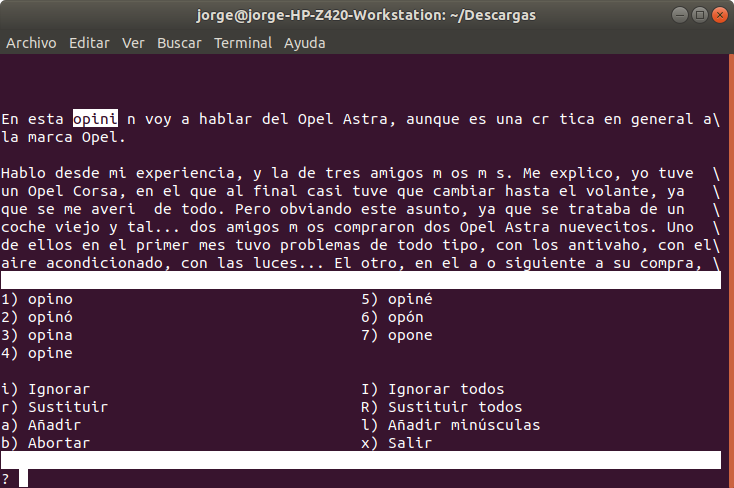
\includegraphics[width=8cm]{aspell.png}
\caption{Vista de la consola interactica de Aspell en Ubuntu con el texto provisto en \textbf{no\_2\_9.txt}}
\end{figure}

Cabe considerar que solo estamos considerando los resultados obtenidos en solo una de las rese\~nas, y si se consideraran todas las rese\~nas probablemente se esperarian resultados similares o peores con nuestro corrector ortogr\'afico que con el de Aspell que esta mucho m\'as optimizado para esta tarea.\newline

\textbf{Posibles mejoras al corrector ortogr\'afico}\newline
Una primera mejora que se le puede realizar al corrector ortogr\'afico es a la hora de elegir el argumento m\'aximo establecer una mejor manera de seleccionar que solo elegir la primera de las palabras que tengan un empate en su c\'alculo.\newline

Una segunda opci\'on es ampliar el Corpus de frecuencias usando palabras mas acorde al contexto al que intentamos corregir, ya que debido a esto algunas palabras que son frecuentes en un contexto no lo son en otro, como fue el caso del Corpus de la RAE que no esta espec\'ificado para el tipo de contexto de opini\'on que requerimos para corregir los textos de rese\~na que estamos evaluando.\newline

Otra opci\'on es utilizar otro tipo de m\'etrica para el string distance. Sin embargo, dependiendo de los contextos de los textos a evaluar un cambio de m\'etrica puede generar una peor correcci\'on que la estamos considerando, adem\'as de que computacionalmente puede ser m\'as pesada la alternativa.\newline

Un par de opciones mas ser\'ian hacer uso del contexto del texto, es decir usar x palabras hacia adelante y hac\'ia atr\'as para establecer una mejor manera de elegir entre las palabras con probabilidad m\'axima igual, y jugar con las probabilidades asignadas a distribuci\'on apriori para generar desempates en las palabras con probabilidad m\'axima igual.
\end{document}